\documentclass[11pt]{article}

% ==== Paquetes ====
\usepackage[utf8]{inputenc}
\usepackage[spanish]{babel}
\usepackage[T1]{fontenc}
\usepackage{amsmath, amssymb, amsfonts, siunitx}
\usepackage{graphicx}
\usepackage{float}
\usepackage{xcolor}
\usepackage{hyperref}
\usepackage{caption}
\usepackage{subcaption}
\usepackage{geometry}
\usepackage{listings}
\usepackage{pdfpages}
\usepackage{tikz}

\definecolor{codegreen}{rgb}{0,0.6,0}
\definecolor{codegray}{rgb}{0.5,0.5,0.5}
\definecolor{codepurple}{rgb}{0.58,0,0.82}
\definecolor{backcolour}{rgb}{0.95,0.95,0.92}

\lstset{
  inputencoding=utf8,
  extendedchars=true,
  literate=
   {á}{{\'a}}1 {é}{{\'e}}1 {í}{{\'i}}1 {ó}{{\'o}}1 {ú}{{\'u}}1
   {Á}{{\'A}}1 {É}{{\'E}}1 {Í}{{\'I}}1 {Ó}{{\'O}}1 {Ú}{{\'U}}1
   {ñ}{{\~n}}1 {Ñ}{{\~N}}1
   {¿}{{?`} }1 {¡}{{!`} }1
}

\lstdefinestyle{mystyle}{
    backgroundcolor=\color{backcolour},   
    commentstyle=\color{codegreen},
    keywordstyle=\color{magenta},
    numberstyle=\tiny\color{codegray},
    stringstyle=\color{codepurple},
    basicstyle=\ttfamily\footnotesize,
    breakatwhitespace=false,         
    breaklines=true,                 
    captionpos=b,                    
    keepspaces=true,                 
    numbers=left,                    
    numbersep=5pt,                  
    showspaces=false,                
    showstringspaces=false,
    showtabs=false,                  
    tabsize=2,
    upquote=true,
    inputencoding=utf8,
}

\lstset{style=mystyle}

\geometry{margin=2.5cm}

% ==== Datos de la tarea ====
\title{IEE3584 - Procesamiento Avanzado de Señales \\
Tarea 7}
\author{Nicolás Seguel}
\date{Septiembre 2025}

\begin{document}

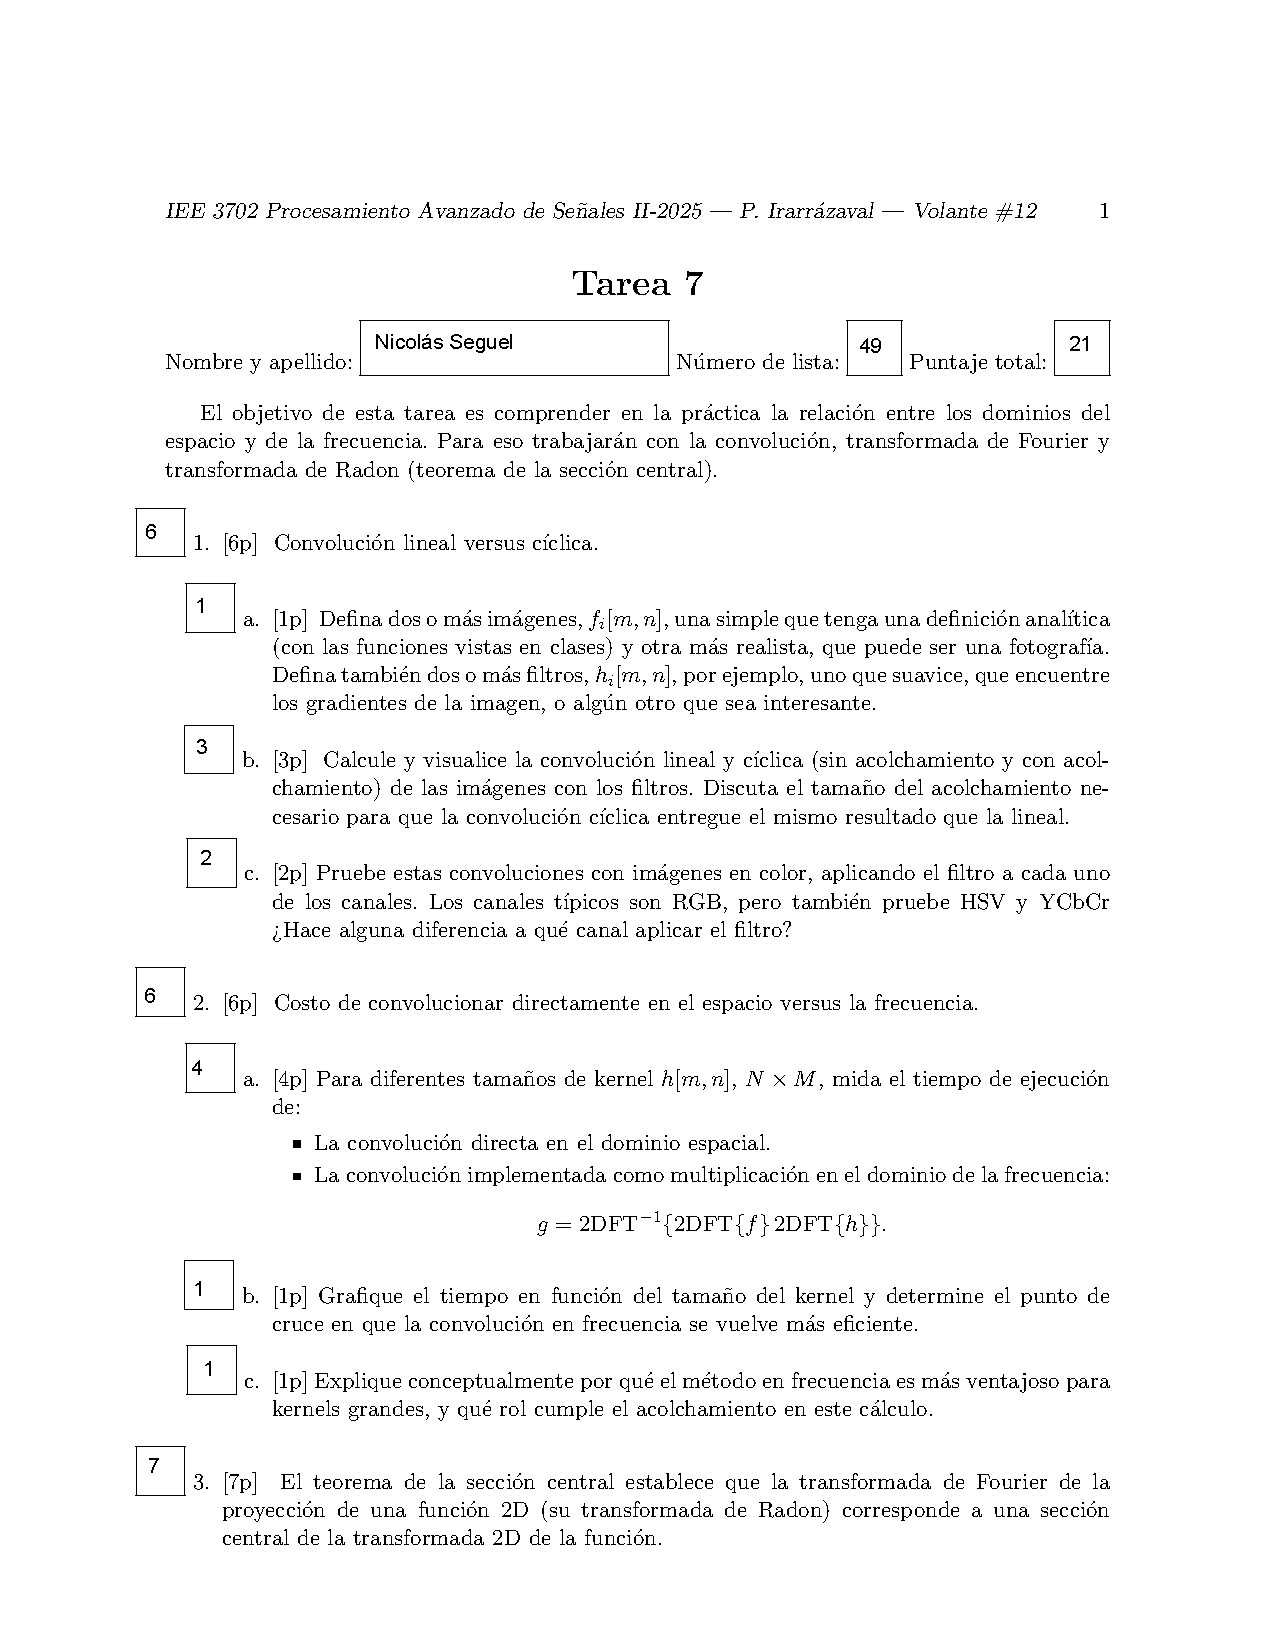
\includepdf[pages=-]{12.tarea07.pdf}
\maketitle

% ==== PREGUNTA 1 ====
\section*{1. Convolución lineal vs cíclica}

\subsection*{a) Imagenes a utilizar}
Se utilizará una imagen real y una imagen binaria simple, que corresponde a un circulo blanco. Los filtro a utilizar son un filtro pasa bajos ideal, es decir, un cuadrado de 25x25 con valores iguales a $\frac{1}{25^2}$, y un filtro de Sobel para detección de bordes.

\subsection*{b) Convolución lineal y cíclica}

Se aplica la convolución lineal y cíclica a la imagen en escala de grises, utilizando ambos filtros.

\begin{figure}[H]
    \centering
    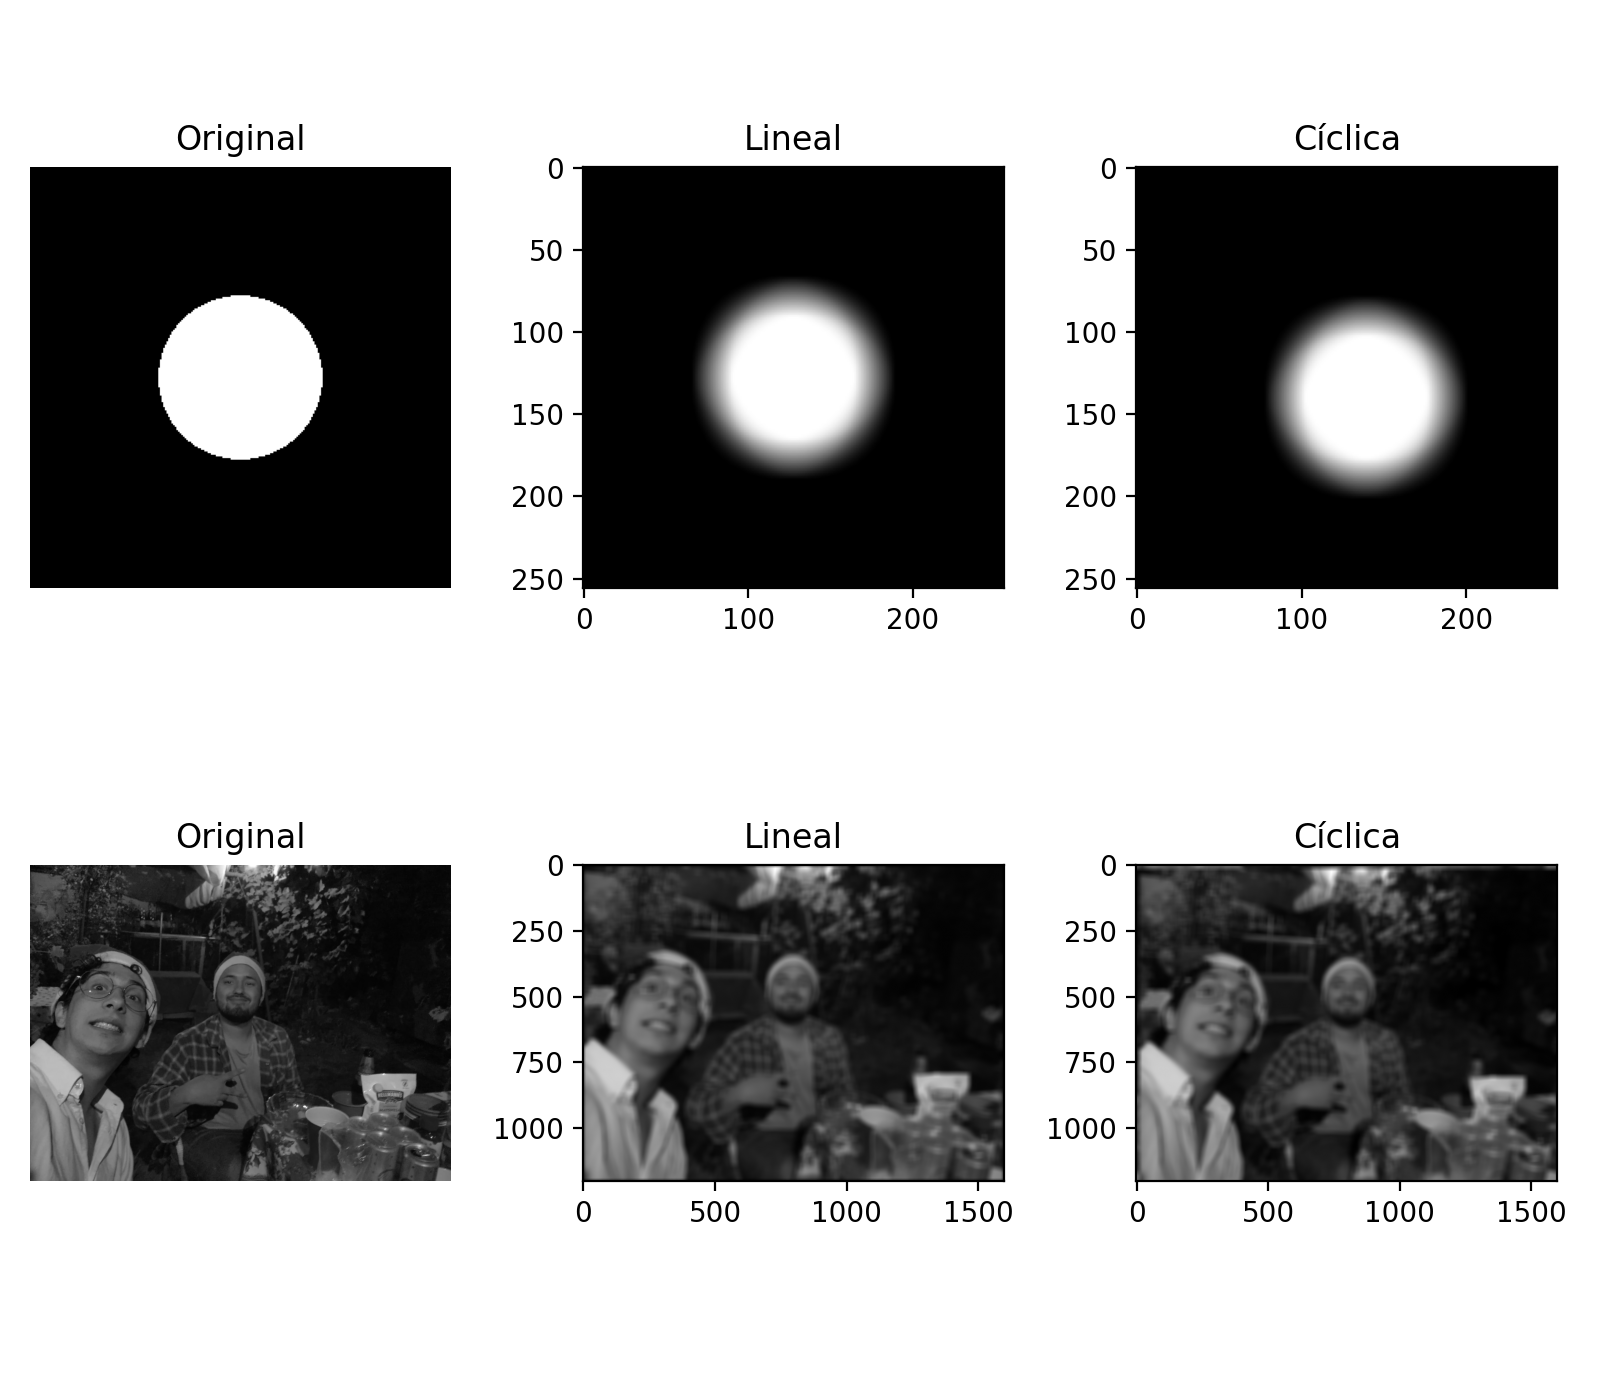
\includegraphics[width=0.85\textwidth]{figs/p1_convolucion_suave.png}
    \caption{Resultados de la convolución lineal y cíclica con un filtro pasa bajos.}
\end{figure}

\begin{figure}[H]
    \centering
    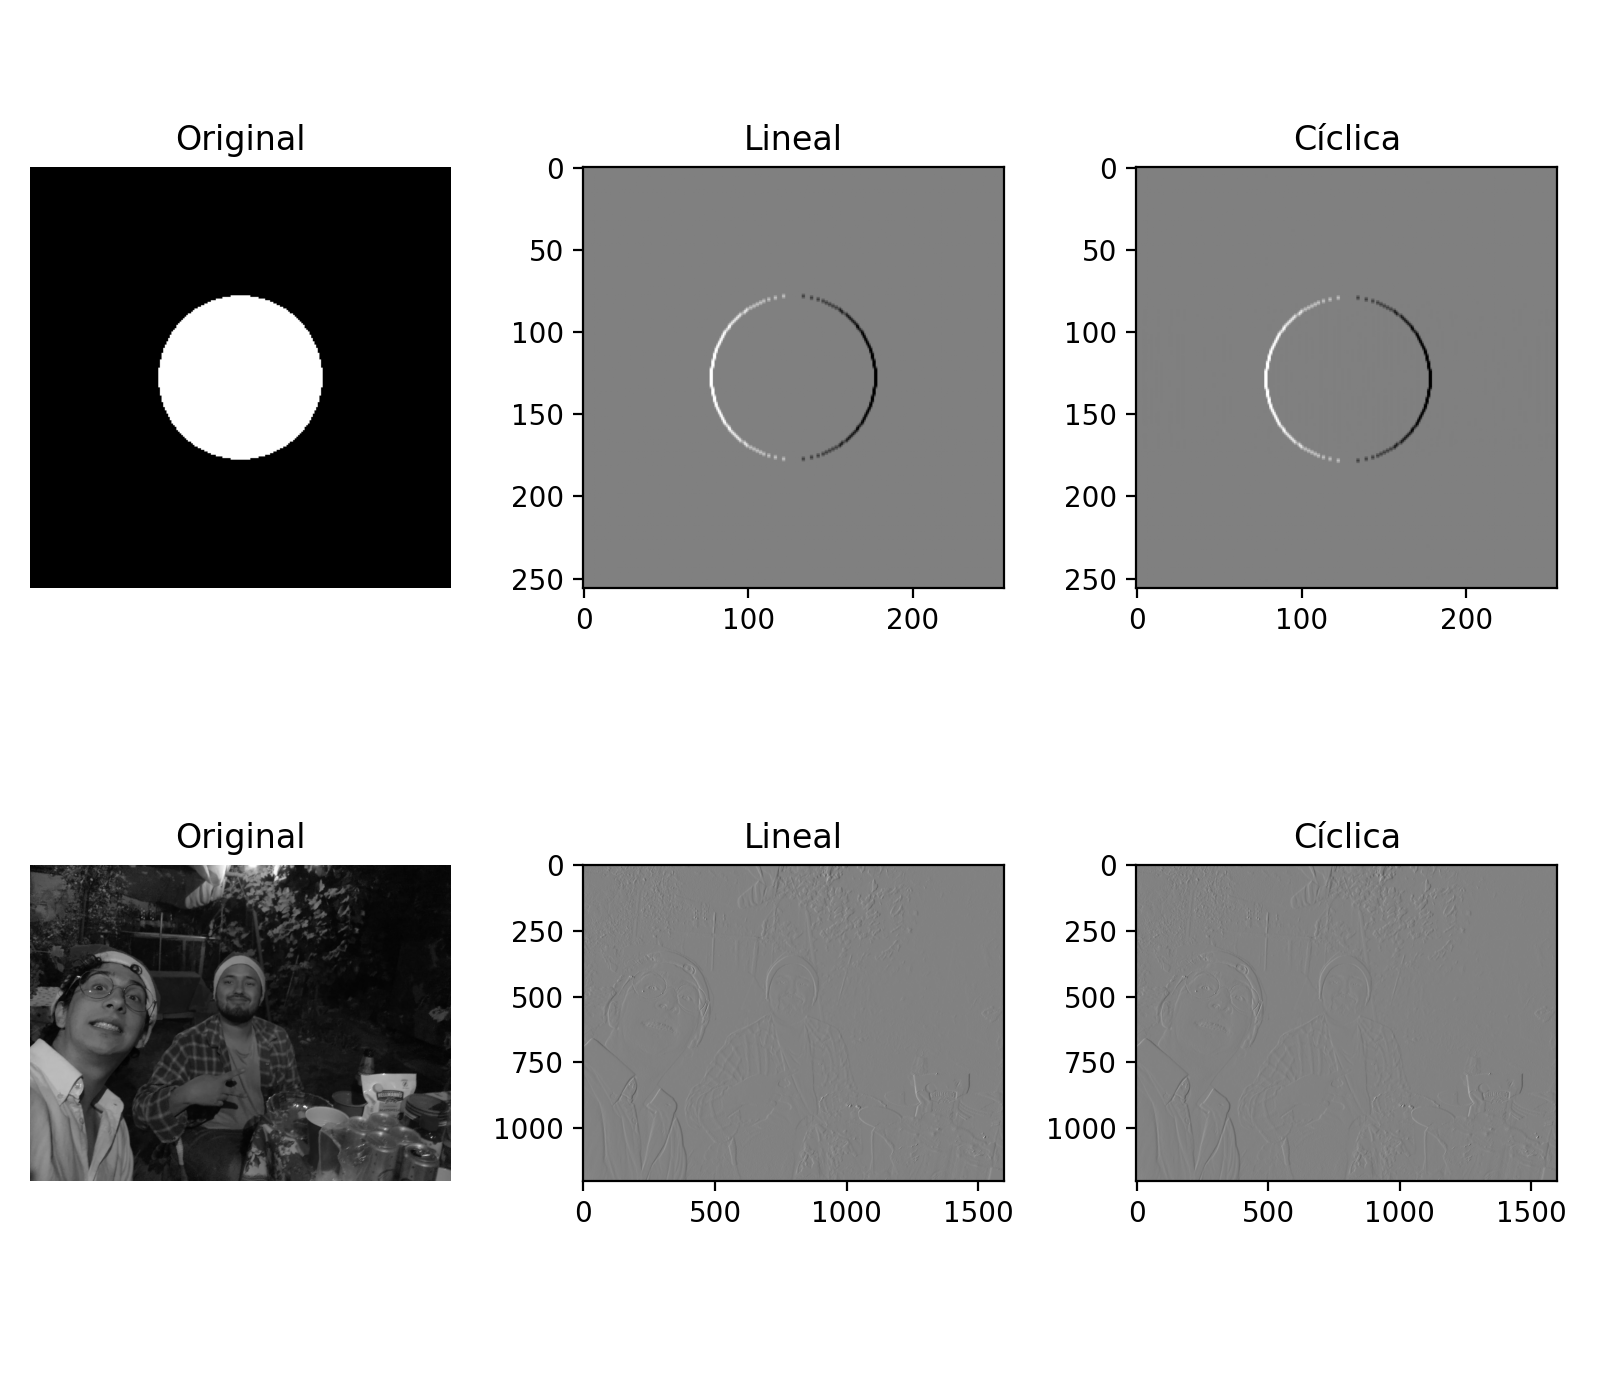
\includegraphics[width=0.85\textwidth]{figs/p1_convolucion_sobel.png}
    \caption{Resultados de la convolución lineal y cíclica con un filtro de Sobel.}
\end{figure}

Se puede ver que la convolución cíclica introduce un efecto de borde en las imagenes. Mientras más grande el tamaño de la máscara, más evidente es este efecto. Si se desea evitar este efecto en la convolución cíclica, se puede aplicar un padding a la imagen original. Esto se debe a que el padding agrega un borde adicional que reduce la interferencia entre los bordes de la imagen original y las copias generadas por la naturaleza de la convolución cíclica.

\subsection*{c) Convoluciones en canales RGB, HSV y YCbCr}

\begin{figure}
    \centering
    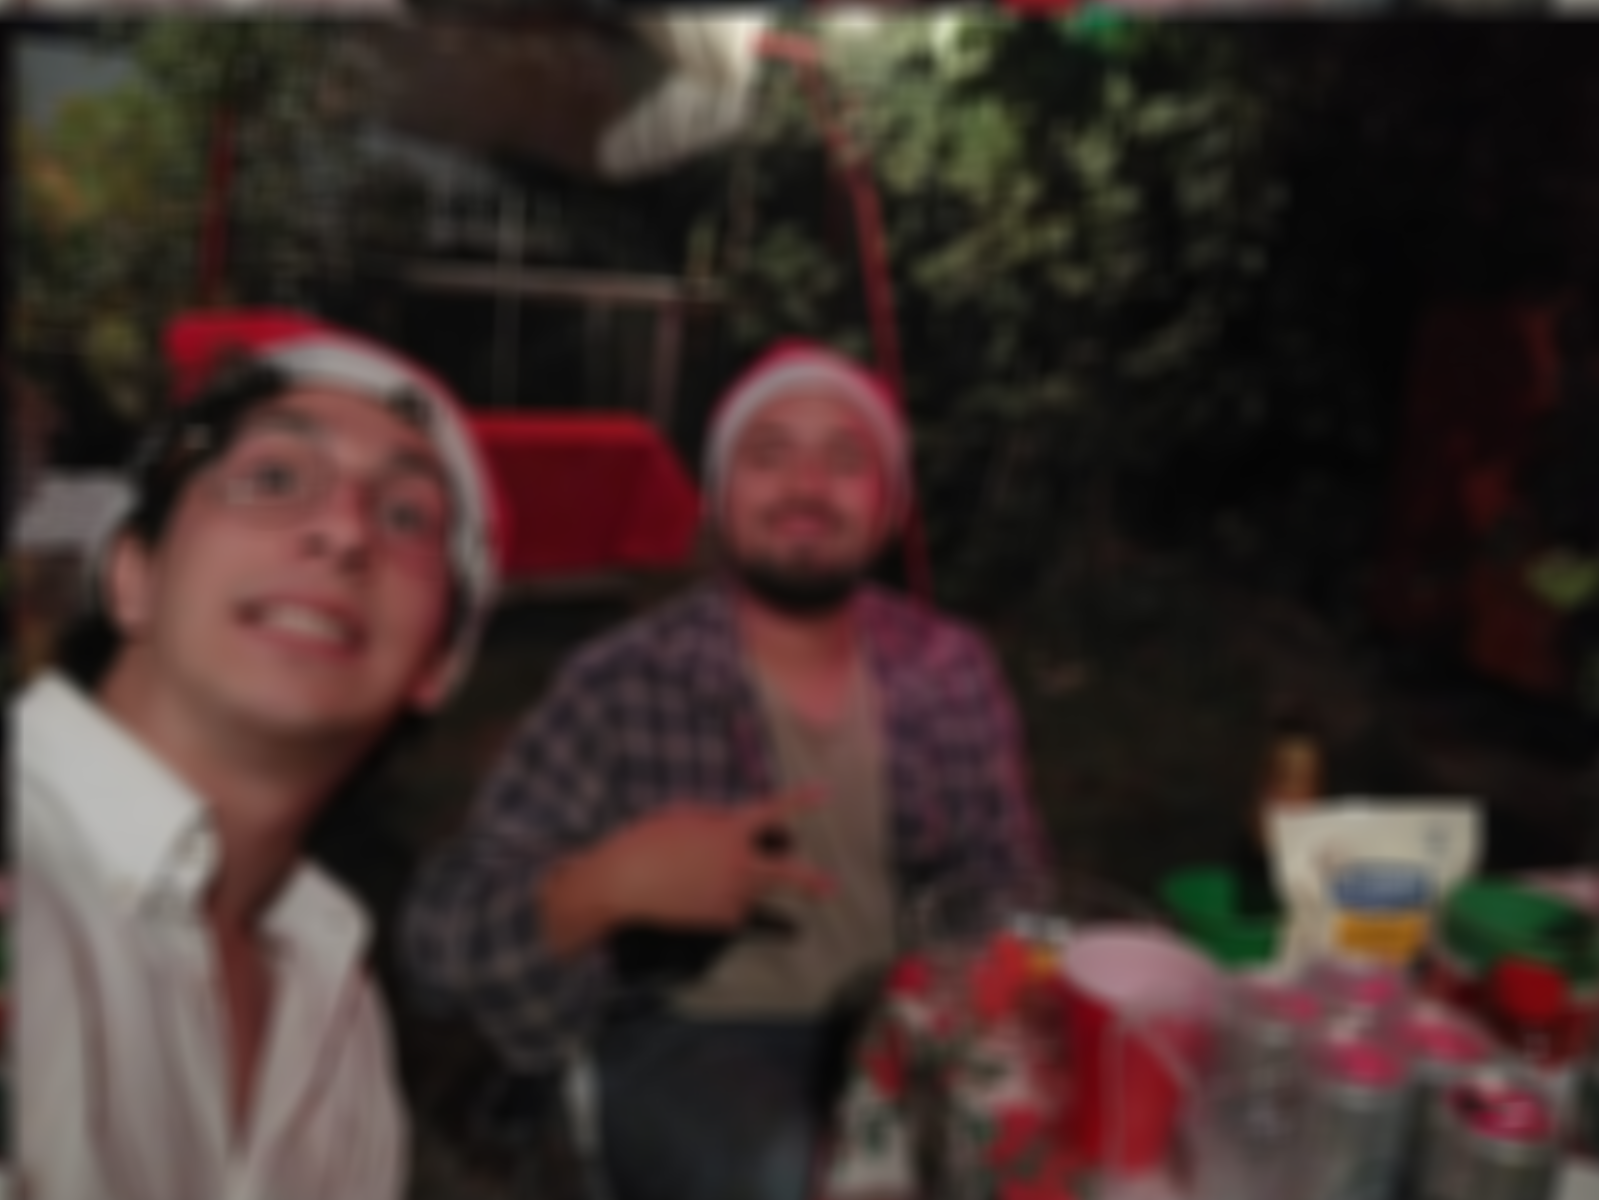
\includegraphics[width=0.32\textwidth]{figs/p1_convolucion_rgb.png}
    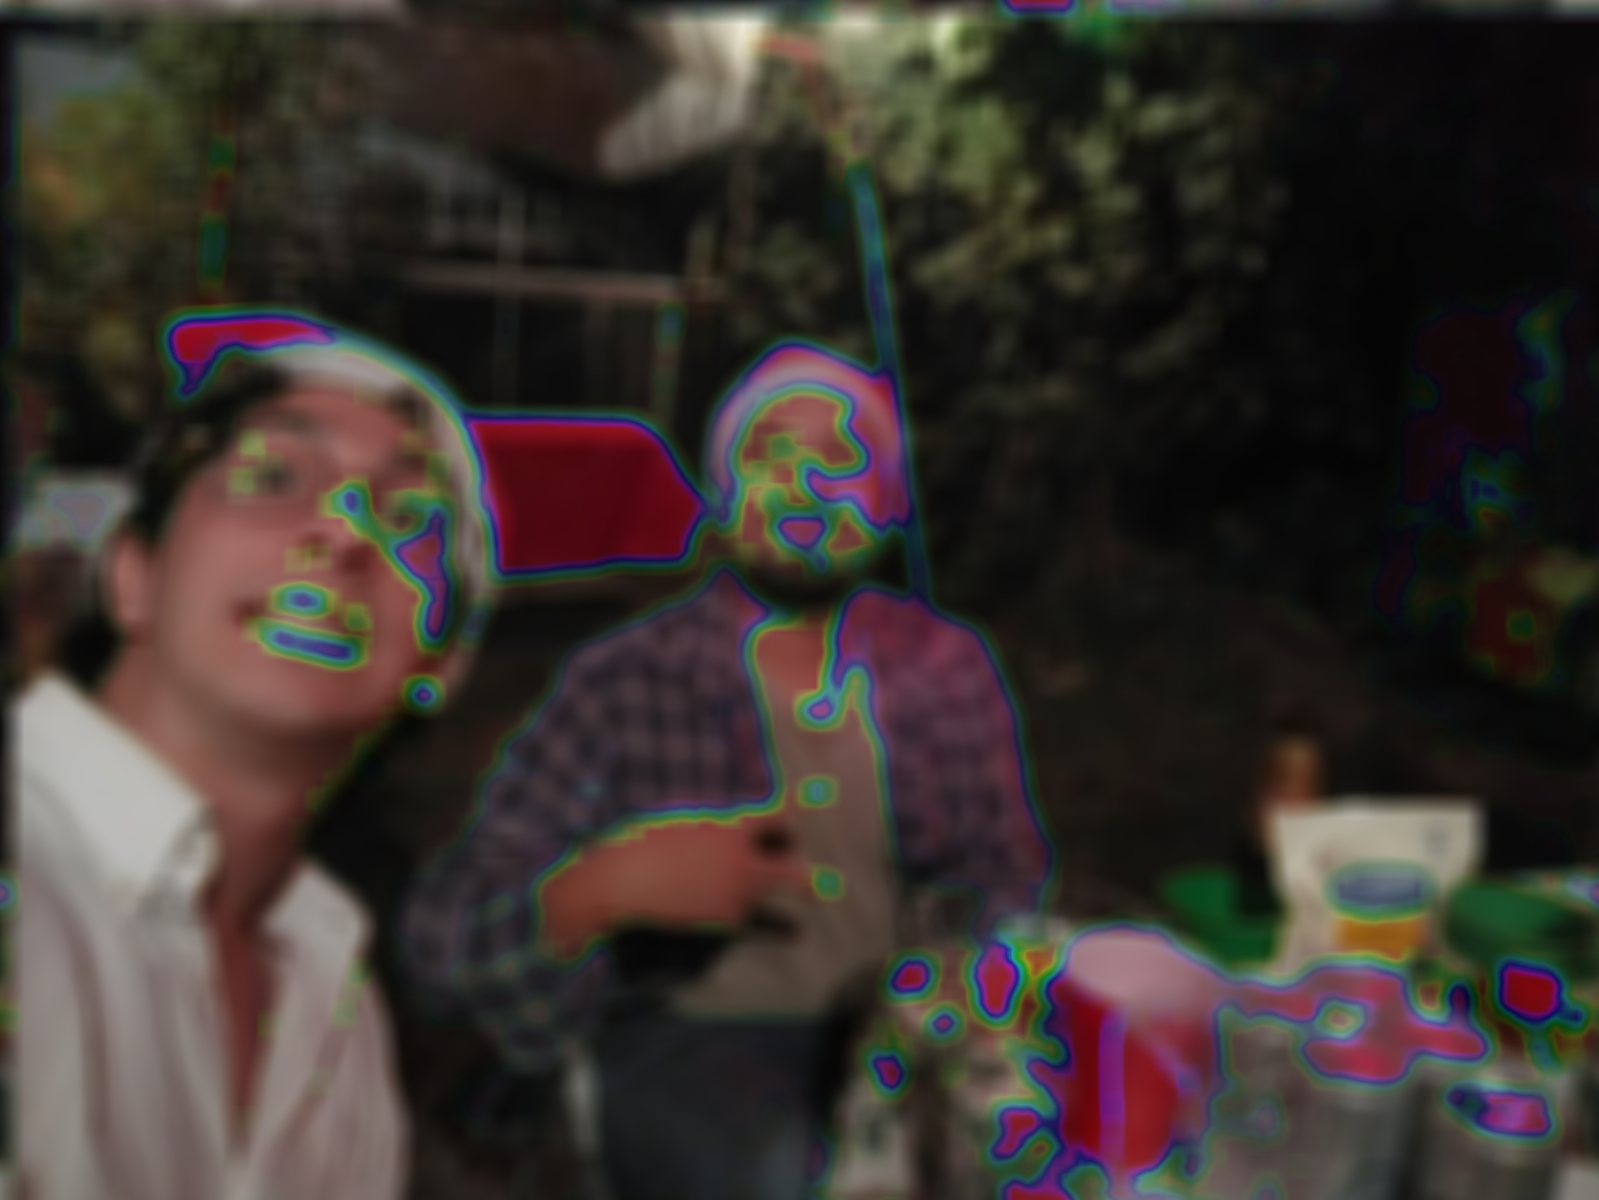
\includegraphics[width=0.32\textwidth]{figs/p1_convolucion_hsv.png}
    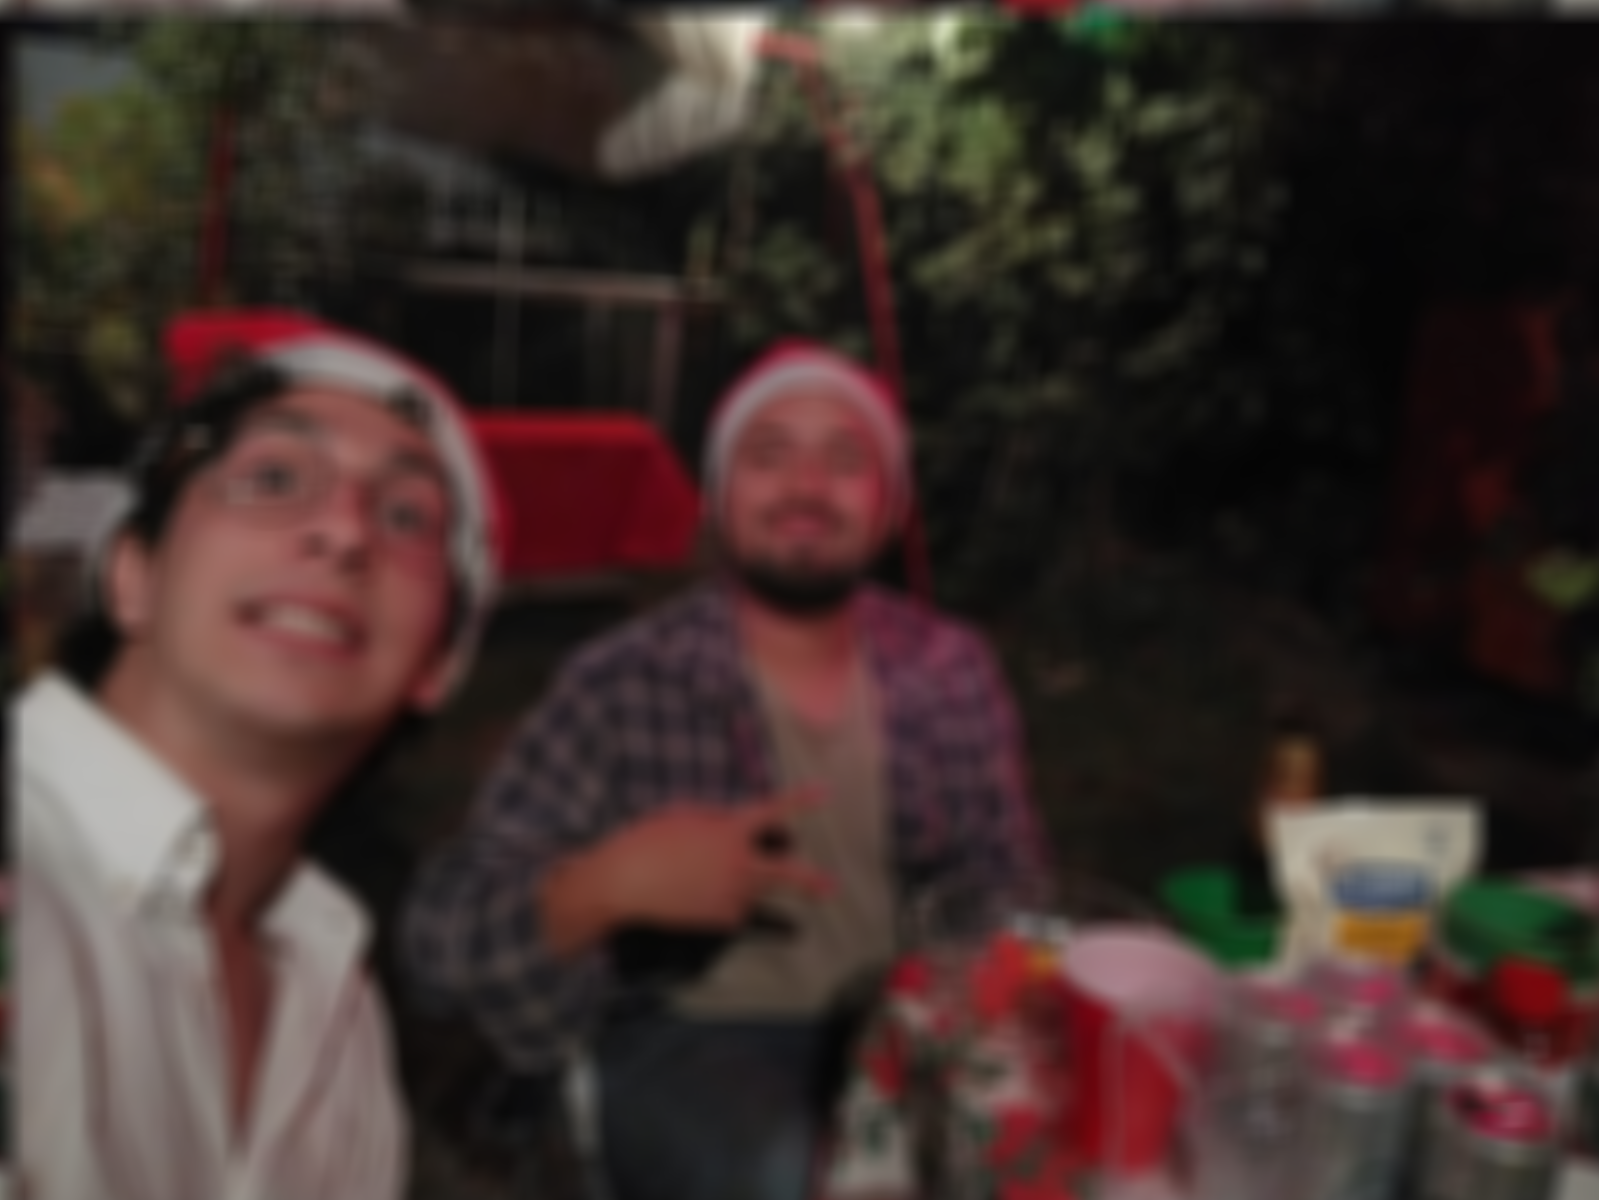
\includegraphics[width=0.32\textwidth]{figs/p1_convolucion_ycbcr.png}
    \caption{Resultados de la convolución cíclica en espacios RGB, HSV y YCbCr.}
\end{figure}

La convolución en el espacio HSV afecta los colores de la imagen, ya que el canal de saturación y valor se ven modificados.

\lstinputlisting[language=Python, caption={p1\_convolucion\_lineal\_vs\_ciclica.py}, label={lst:p1}]{src/p1_convolucion_lineal_vs_ciclica.py}

% ==== PREGUNTA 2 ====
\section*{2. Costo computacional de la convolución}

\subsection*{a) Convolución espacial y frecuencial}

Para distintos tamaños del kernel (de $3\times3$ a $255\times255$), se mide el tiempo de ejecución con \texttt{time.time()}.

\begin{figure}
    \centering
    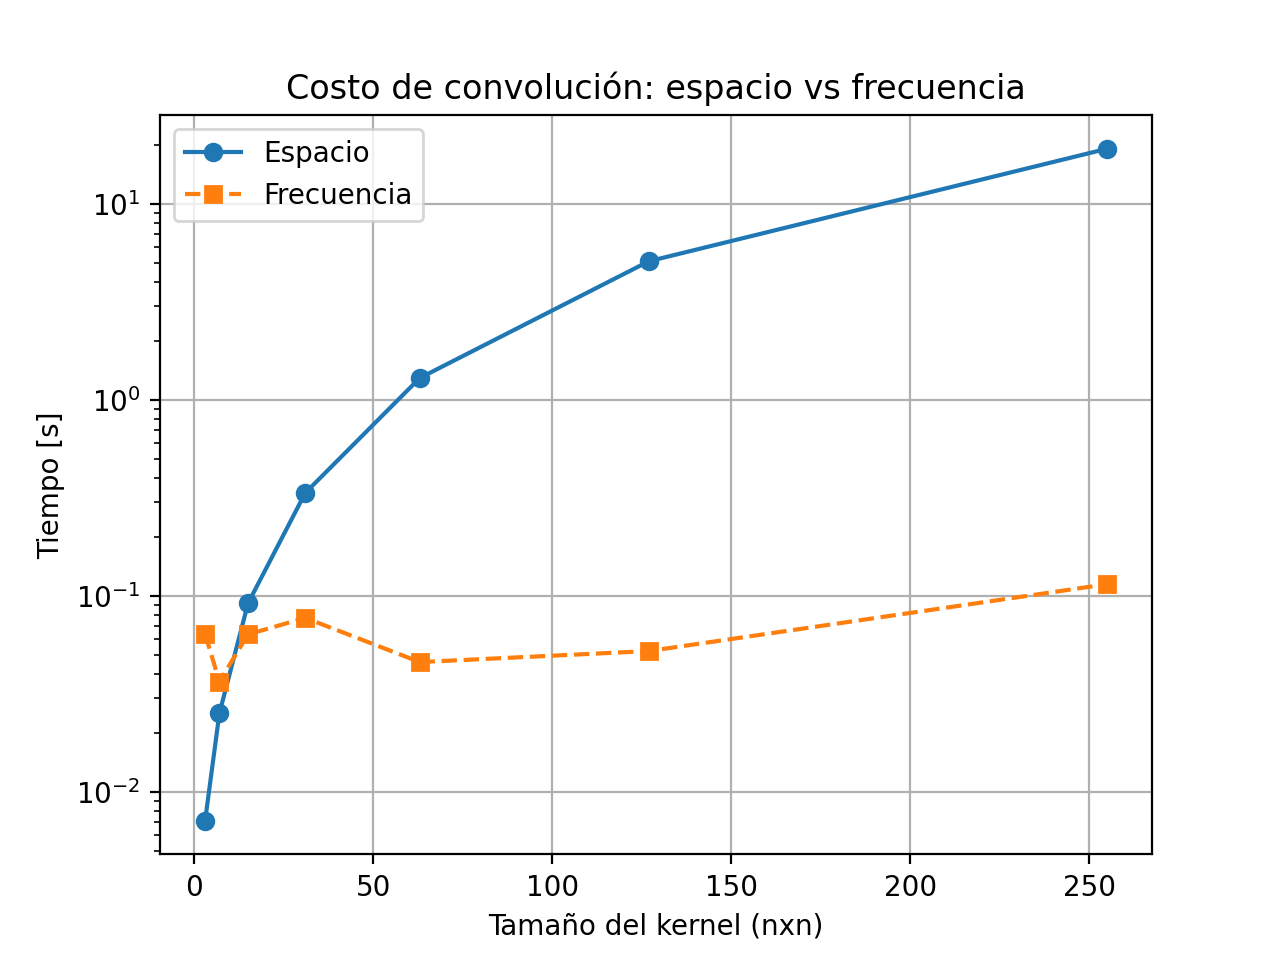
\includegraphics[width= 0.8\textwidth]{figs/p2_tiempos_convolucion.png}
    \caption{Costo computacional de la convolución espacial y frecuencial en función del tamaño del filtro.}
\end{figure}

\subsection*{b) Tiempos de ejecución}
El gráfico anterior muestra que la convolución en el dominio espacial es más eficiente para tamaños de kernel pequeños, mientras que la convolución en el dominio frecuencial se vuelve más eficiente a medida que el tamaño del kernel aumenta. El punto de cruce entre ambas curvas esta cerca de un tamaño de kernel de $10\times10$.

\subsection*{c) Ventaja de la convolución en frecuencia}

La convolución en espacio calcula el producto punto entre el kernel y la región de la imagen para cada píxel, lo que implica un costo computacional que crece con el tamaño del kernel. En contraste, la convolución en frecuencia utiliza la Transformada Rápida de Fourier (FFT) para transformar tanto la imagen como el kernel al dominio frecuencial, donde la convolución se realiza mediante una multiplicación punto a punto. La FFT tiene un costo computacional de $O(N \log N)$, lo que la hace más eficiente para kernels grandes.

\lstinputlisting[language=Python, caption={p2\_costo\_convolucion.py}, label={lst:p2}]{src/p2_costo_convolucion.py}

% ==== PREGUNTA 3 ====
\section*{3. Teorema de la Sección Central}

\subsection*{a) Transformada de Fourier y Radon}
Se genera una imagen analítica formada por un rectángulo, sobre la cual se calcula:
\begin{itemize}
    \item La transformada de Fourier 2D.
    \item La transformada de Radon en distintos ángulos.
\end{itemize}

\begin{figure}[H]
    \centering
    
\includegraphics[width=0.3\textwidth]{figs/p3_imagen_base.png}
    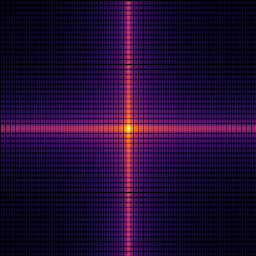
\includegraphics[width=0.3\textwidth]{figs/p3_fourier2d.png}
    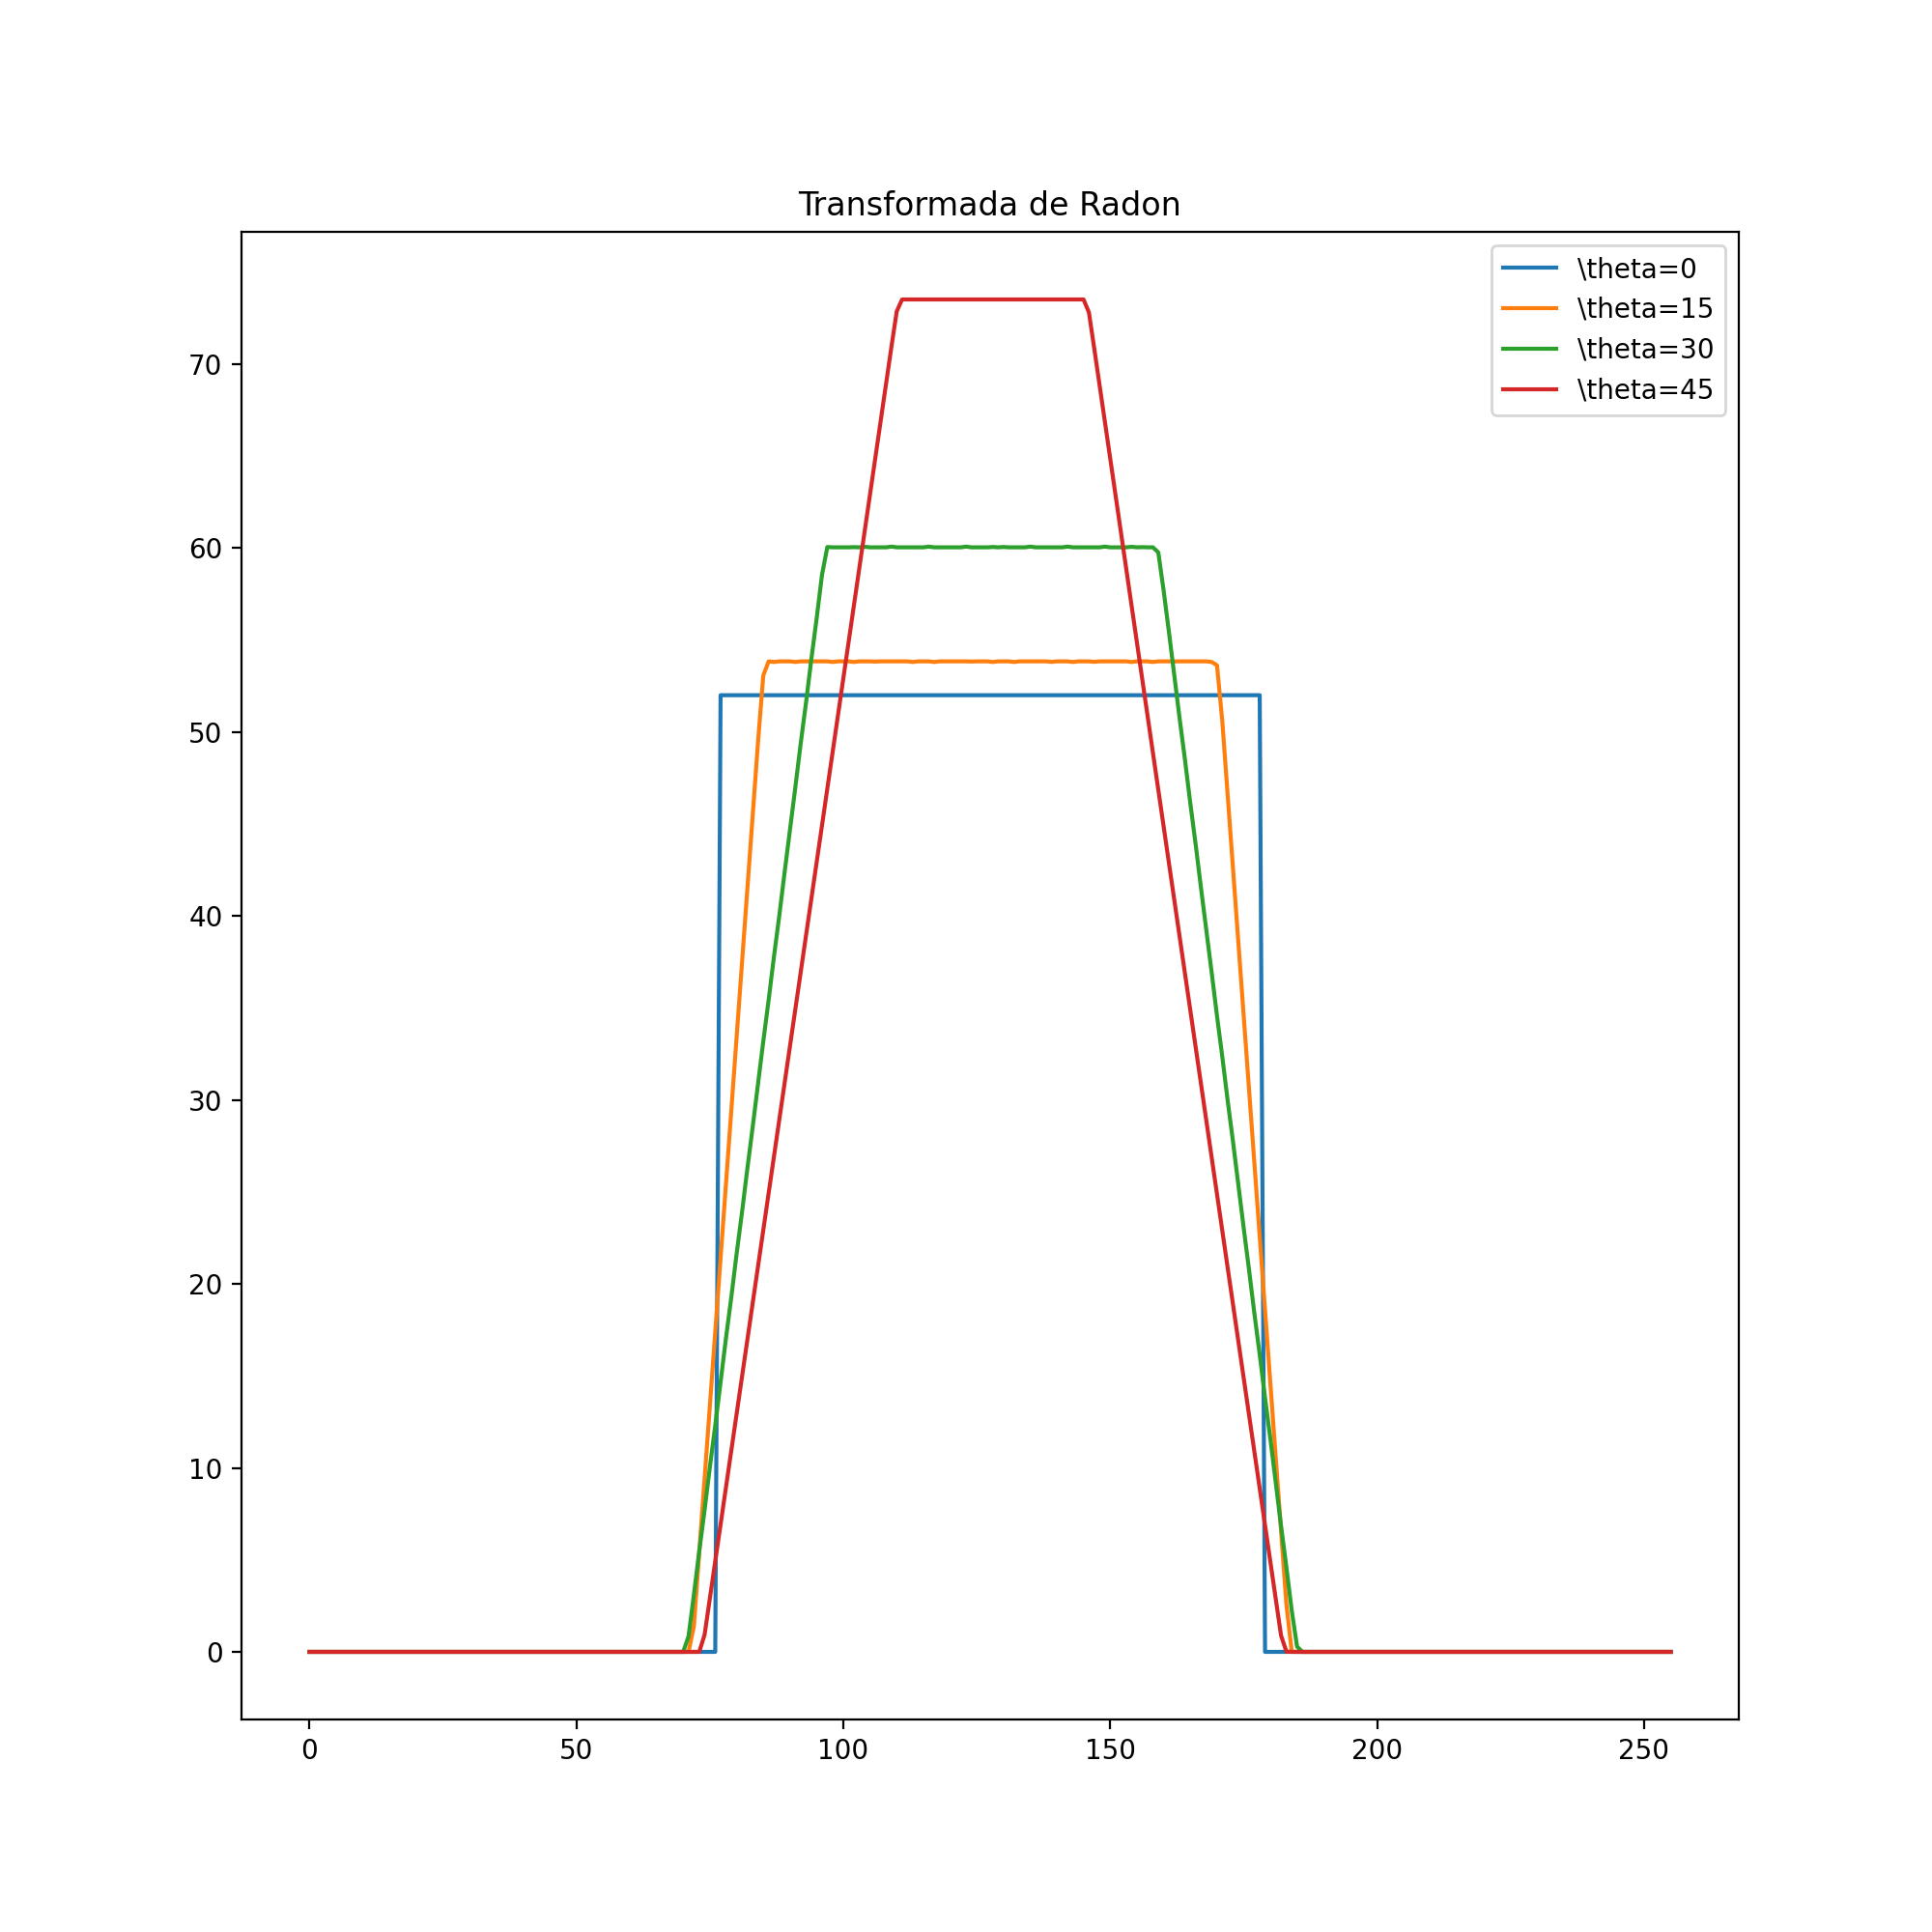
\includegraphics[width=0.3\textwidth]{figs/p3_radon.png}
    \caption{Imagen base, transformada de Fourier 2D y transformada de Radon.}
\end{figure}

\subsection*{b) Comparación de secciones}
Se compara la transformada de Fourier de las proyecciones de Radon con las secciones centrales de la transformada 2D, verificando el teorema de la sección central.

\begin{figure}[H]
    \centering
    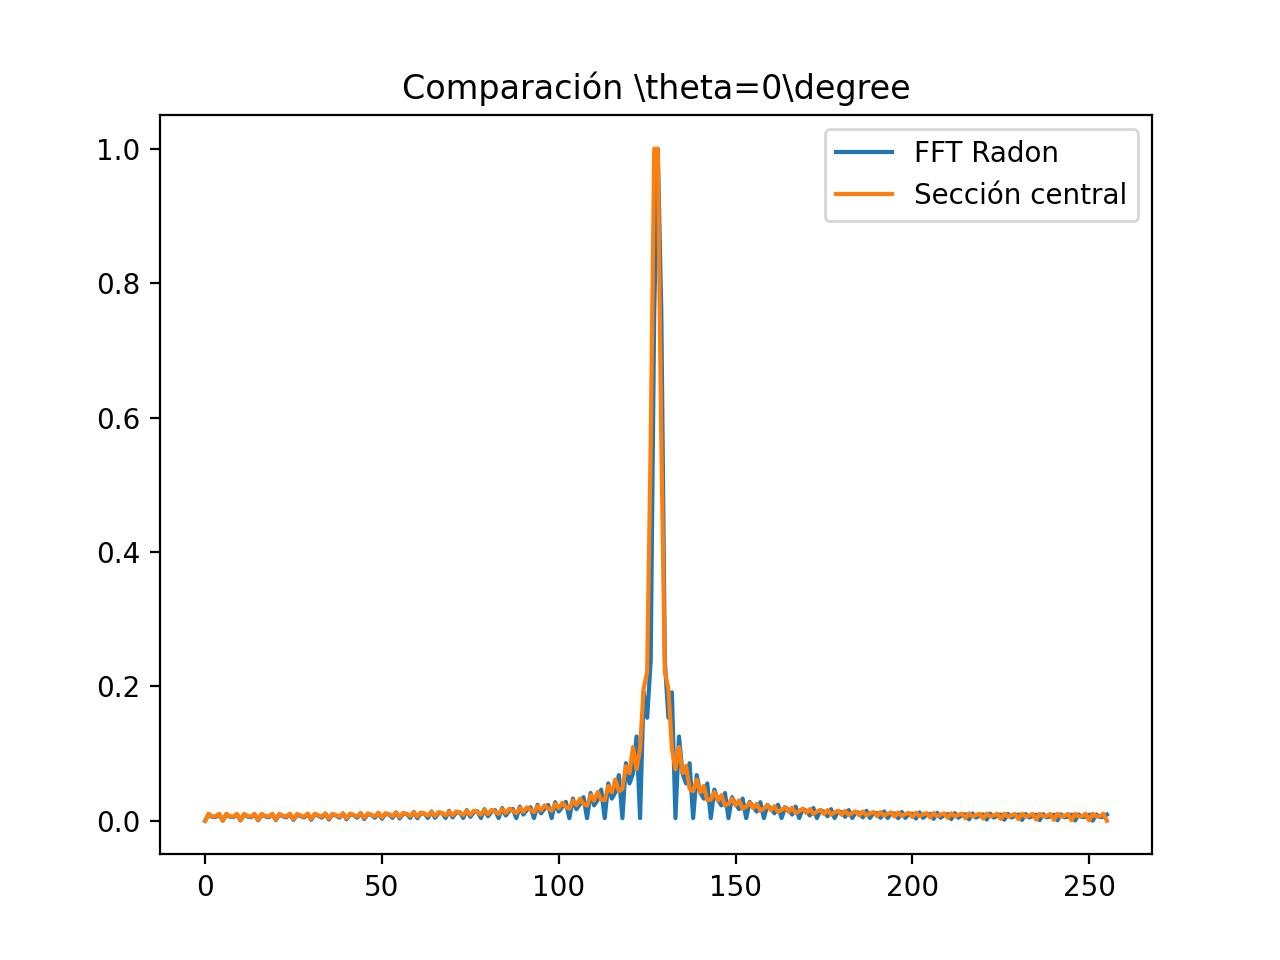
\includegraphics[width=0.6\textwidth]{figs/p3_comparacion_theta0.png}
    \caption{Ejemplo de comparación entre la FFT de Radon y la sección central del espectro.}
\end{figure}

\subsection*{c) Resultados}

\begin{figure}[H]
    \centering
    
\includegraphics[width= 0.45\textwidth]{figs/p3_imagen_base.png}
    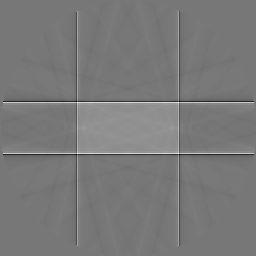
\includegraphics[width= 0.45\textwidth]{figs/p3c_recon_iradon.png}
    \caption{Imagen base y reconstrucción mediante retroproyección filtrada.}
\end{figure}

La reconstrucción mediante retroproyección filtrada a partir de las proyecciones de Radon se asemeja bastante a la imagen original. Sin embargo, se observa lineas que se extienden a lo largo de los bordes del bloque, además de una difuminación en el color de la imagen. Esto se debe a la falta de angulos en la transformada de Radon, lo que genera artefactos en la reconstrucción.

\lstinputlisting[language=Python, caption={p3\_teorema\_seccion\_central.py}, label={lst:p3}]{src/p3_teorema_seccion_central.py}

% ==== PREGUNTA 4 ====
\section*{4. Ciclo Abel-Fourier-Hankel}

\subsection*{b) Gráficos de la transformada}

\begin{figure}[H]
    \centering
    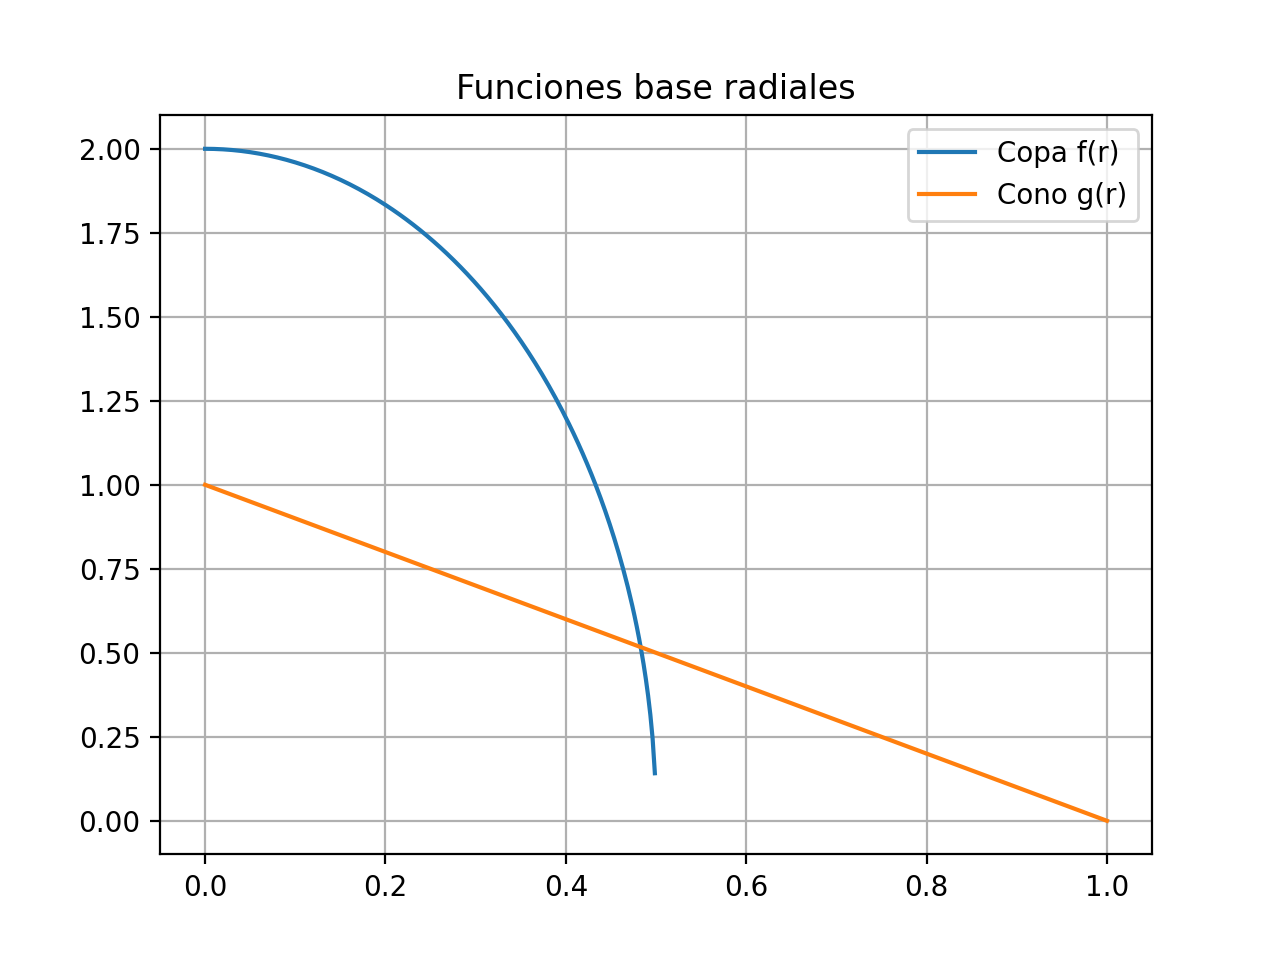
\includegraphics[width=0.48\textwidth]{figs/p4_funciones_base.png}
    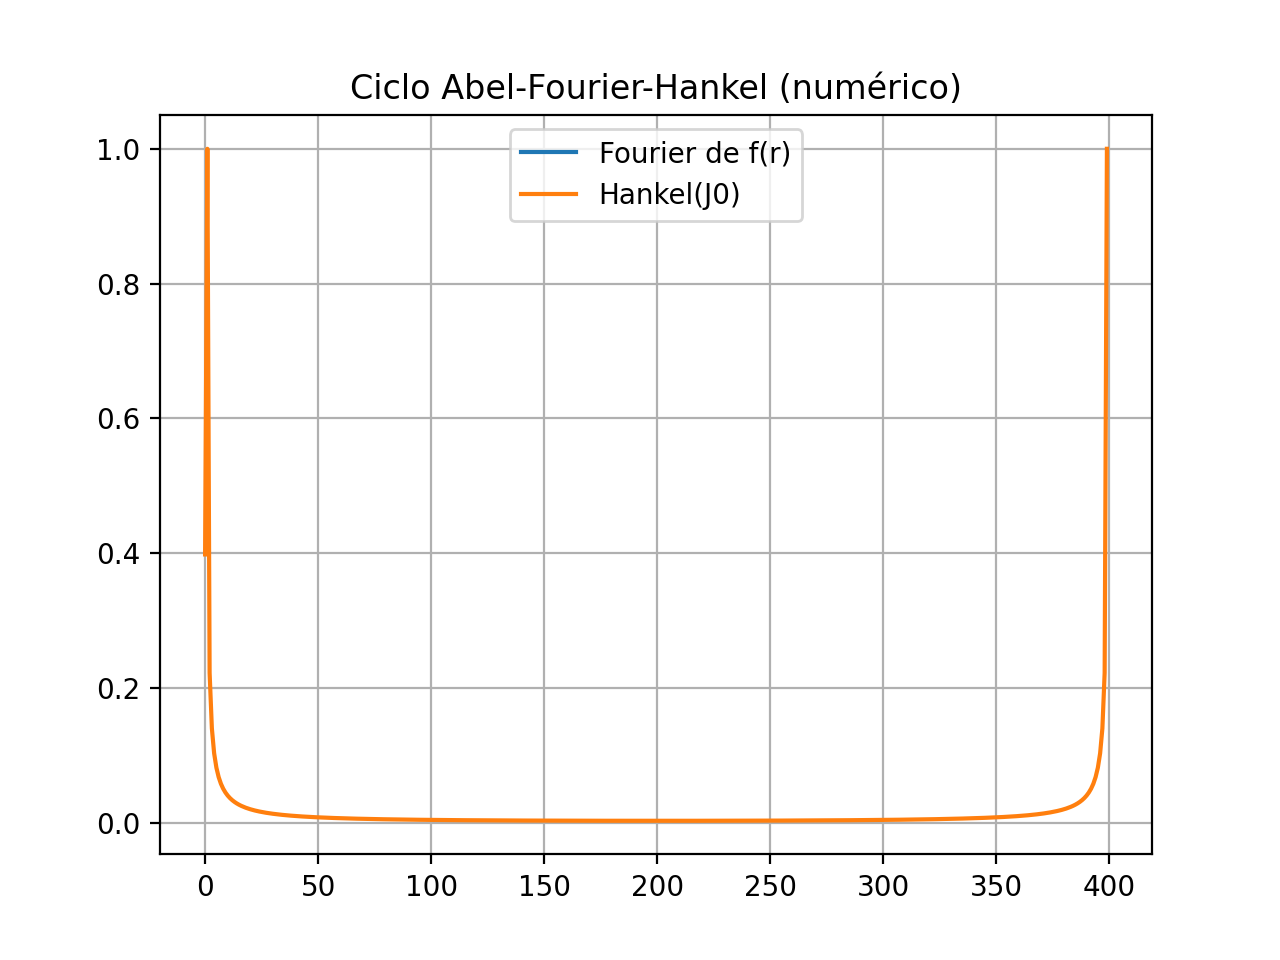
\includegraphics[width=0.48\textwidth]{figs/p4_ciclo_afh.png}
    \caption{Funciones base radiales y comparación de sus transformadas en el ciclo AFH.}
\end{figure}

\lstinputlisting[language=Python, caption={p4\_abel\_fourier\_hankel.py}, label={lst:p4}]{src/p4_abel_fourier_hankel.py}

\end{document}